\documentclass{article}
\usepackage[utf8]{inputenc}
\usepackage{enumitem}
\setlist[itemize]{topsep=2pt, parsep=2pt, itemsep=2pt}
\setlist[enumerate]{topsep=2pt, parsep=2pt, itemsep=2pt}
\usepackage[numbers,sort&compress]{natbib}
\usepackage{graphicx}
\usepackage{textcomp}
\usepackage{amsmath}
\usepackage{amssymb}
\usepackage{newunicodechar}
\usepackage{tikz}
\usetikzlibrary{arrows.meta,positioning,shapes,fit}

\usepackage{microtype}
\usepackage{booktabs}
\usepackage{xcolor}
\definecolor{arcblue}{RGB}{0, 102, 204}
\usepackage{titlesec}
\usepackage{setspace}
\usepackage{tcolorbox}
\usepackage[left=1.25in,right=1in,top=1in,bottom=1in]{geometry}
\usepackage{qrcode}

\titleformat{\section}{\large\bfseries\color{arcblue}}{\thesection}{1em}{}
\titleformat{\subsection}{\normalsize\bfseries\color{arcblue}}{\thesubsection}{1em}{}

\newtcolorbox{keypoint}{colback=blue!5!white,colframe=arcblue!75!black,title=Key Takeaway}

\setstretch{1.15}

\usepackage{fancyhdr}
\pagestyle{fancy}
\fancyhf{}
\fancyhead[L]{\textit{Arc: Structured, Concurrent, Provenance-Aware AI Memory}}
\fancyhead[R]{\thepage}
\fancyfoot[C]{\textit{Position Paper}}
\renewcommand{\headrulewidth}{0.4pt}
\renewcommand{\footrulewidth}{0.4pt}

\usepackage[colorlinks=true,linkcolor=arcblue,citecolor=arcblue,urlcolor=cyan]{hyperref}

\newunicodechar{ }{\,}

\title{Arc: Towards Structured, Concurrent, and Provenance-Aware Collective AI Memory for Software Engineering}
\author{%
  Jarrod Barnes\\
  Arc Computer\\
  \texttt{Jarrod@arc.computer}
}
\date{May 2025}
\begin{document}
\maketitle

\begin{center}
\large\textbf{Executive Summary}
\end{center}
\noindent As AI generates exponentially more code, the critical bottleneck in software engineering is shifting from \textit{generation} to \textit{understanding, provenance, and coordination}. Arc addresses this fundamental challenge by transforming every codebase into a continuously evolving world model—a live, executable graph of architecture, rationale, and provenance that both humans and AI agents can query, update, and learn from. This memory layer is the missing link between today's siloed copilots and tomorrow's coordinated, autonomous software factories. For engineering leaders, Arc delivers increased velocity, enhanced trust through transparent provenance, improved resilience during incidents, and true AI augmentation through contextual awareness. Our initial focus on AI code review provides immediate value while building toward our vision of coordinated multi-agent systems that can safely evolve complex software in parallel.

\vspace{0.5cm}
\begin{abstract}
Despite their ability to resolve real-world GitHub issues and ingest vast context windows, frontier AI coding agents struggle with a "transient-context ceiling"—preserving causal rationale behind long-running changes. Complex software evolution requires memory that is persistent, structured, and supports semantically-aware concurrent modifications.

Arc is an architecture enabling multiple reinforcement learning agents to collaboratively manage codebases as continuously-evolving world models through three integrated components: (i) \textbf{Temporal Knowledge Graphs (TKGs)} providing structured, queryable history of code artifacts and decisions; (ii) \textbf{Causal CRDT layer} extending Conflict-free Replicated Data Types with semantic invariant checks derived from the TKG; and (iii) \textbf{Provenance-Driven RL} rewarding agents for generating and consuming causal context, fostering coordination and auditable reasoning.

This approach transforms memory from passive retrieval into an active, shared world model for both human and AI developers. We outline the Arc architecture, introduce the SYNAPSE benchmark for empirical validation, and present a research agenda for this critical challenge in AI-assisted software engineering.
\end{abstract}

\noindent\textbf{Keywords:} Temporal Knowledge Graphs, Causal CRDTs, Reinforcement Learning, Software Engineering, Multi-Agent Systems, Provenance


\section{Introduction}
Software engineering is undergoing a profound transformation driven by AI-powered code generation \cite{ref1, ref2}. Despite their capabilities, frontier AI coding agents face a critical challenge: preserving causal rationale behind long-running changes. This "transient-context ceiling" persists even with multi-million token contexts, as models struggle to retain deep causal relationships and design rationale over time.

\textbf{North Star.} Arc transforms codebases into continuously-evolving world models—live, executable graphs of architecture, rationale, and provenance that both humans and AI agents can query and update. As AI generates more code, the bottleneck shifts from generation to \textit{understanding, provenance, and coordination}. Arc serves as the essential memory layer for verified provenance and coherent multi-agent collaboration, supporting a paradigm where engineering work evolves from implementation to strategic oversight.

When crucial context—like API design reasoning—is lost, its connection to future edits becomes tenuous, impeding collaborative tasks like security upgrades and cross-language migrations. Complex software evolution demands memory that is \textit{persistent}, \textit{concurrently writable}, and \textit{semantically consistent} with software rules. Without such a substrate, development suffers from duplicated work, integration conflicts, opaque AI decisions, and architectural decay—a phenomenon we term "context collapse."

\textbf{Core Thesis:} Treat the codebase as a living graph of artifacts, dependencies, and decisions, then enforce semantic rules when agents propose changes. With this foundation, we can train agents to act as reliable, accountable teammates, not reckless auto-complete engines. Lifting the transient-context ceiling and addressing the context collapse necessitates the co-design of three pillars:
\begin{enumerate}
    \item \textbf{Remembering History \& Rationale:} Beyond simple file diffs, agents require structured, queryable history. \textbf{Temporal Knowledge Graphs (TKGs)} encode the evolving state of artifacts, design decisions (including ingested Architectural Decision Records - ADRs), requirements, and agent actions, allowing queries like "What requirement led to this API change?" \cite{ref_zep_gh, ref_letta_gh, ref_letta_blog}.
    \item \textbf{Enabling Safe Parallel Work:} To allow concurrent modifications by multiple human and AI actors without breaking code semantics, we propose \textbf{Causal CRDTs}. These generalize Conflict-free Replicated Data Types (CRDTs) with software-specific semantic checks derived from the TKG, preserving crucial dependencies (e.g., build order, API contracts) and preventing logical conflicts \cite{ref16}.
    \item \textbf{Learning from Collective Experience:} To encourage effective coordination, documentation, and accountability, we employ \textbf{Provenance-Driven Reinforcement Learning (RL)}, building on frameworks that synergize reasoning and acting \cite{ref7, ref40_rlgpt}. Agents are rewarded not only for task progress but critically for generating and consuming causal context within the TKG—linking changes to requirements and documenting decisions—thereby fostering auditable and collaborative AI systems.
\end{enumerate}
This paper details the Arc architecture, discusses related work, outlines the SYNAPSE benchmark for empirical validation, and presents a research agenda inviting community collaboration to build this essential memory layer for the future of software engineering.

\begin{keypoint}
Arc transforms every codebase into a continuously-evolving world model—a live, executable graph of architecture, rationale, and provenance that both humans and AI agents can query, update, and learn from.
\end{keypoint}

\begin{figure}[h]
  \centering
  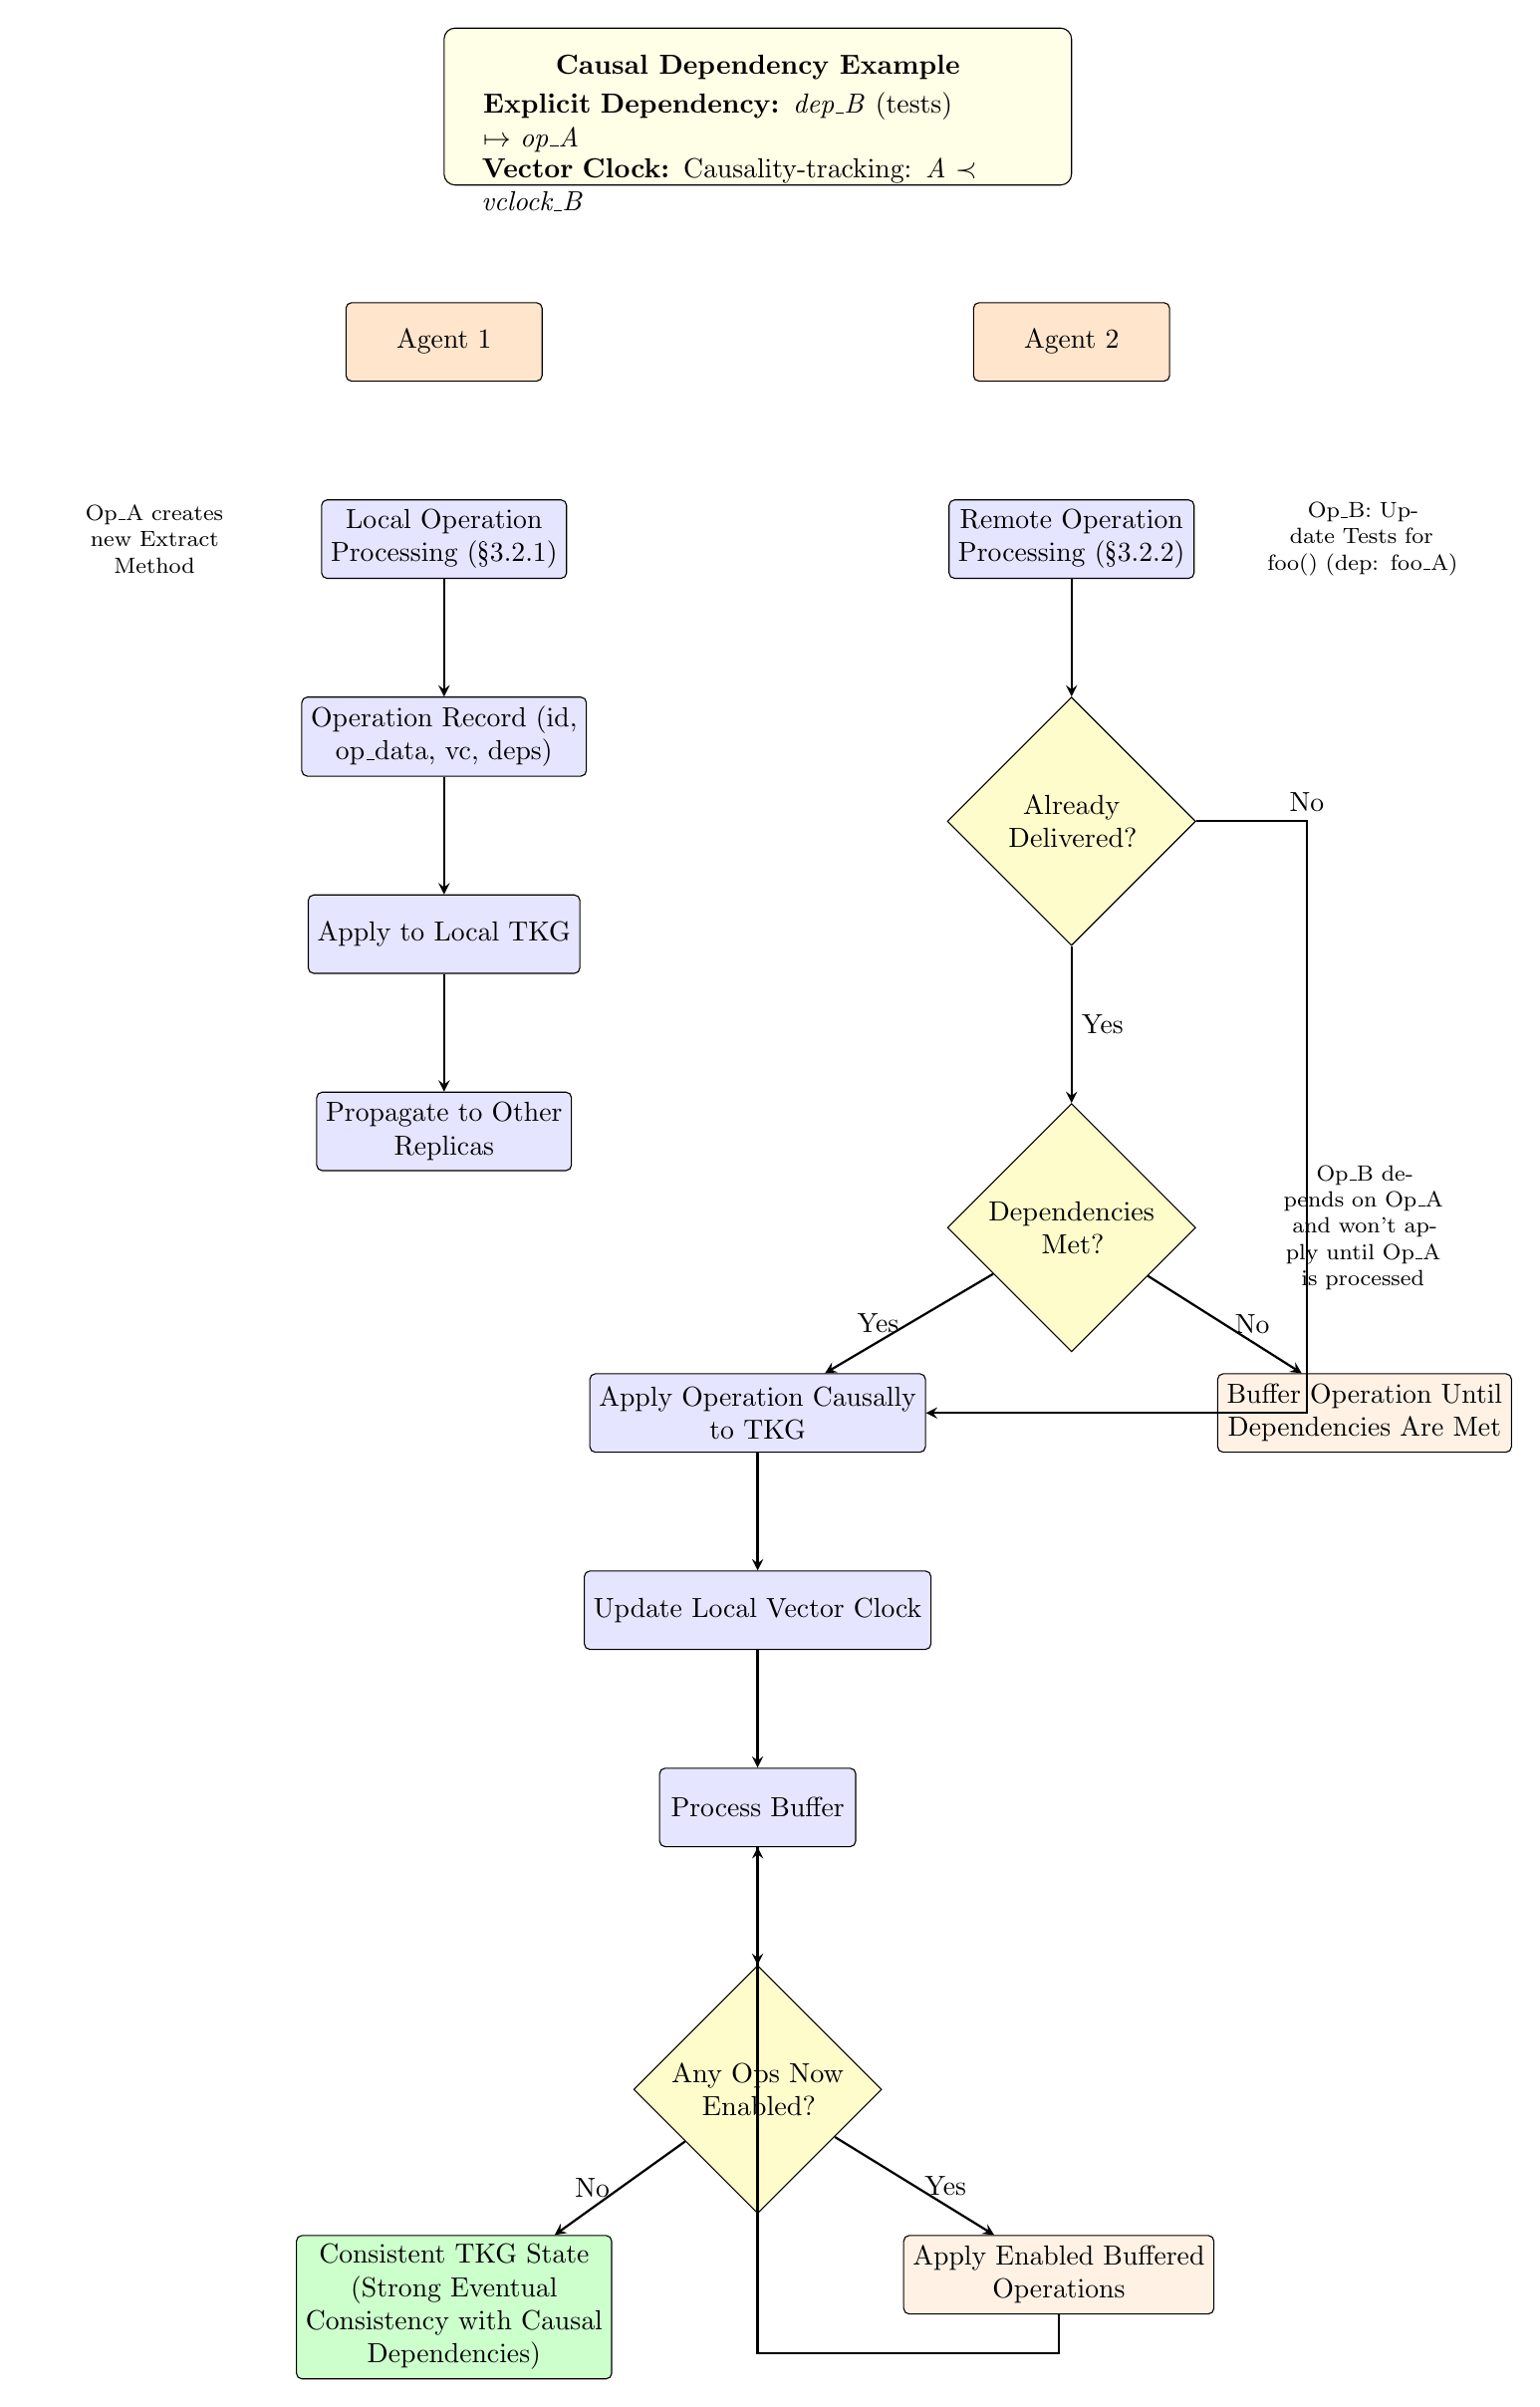
\begin{tikzpicture}[
    node distance=1.5cm and 2cm,
    box/.style={draw, minimum width=2.5cm, minimum height=1cm, align=center, rounded corners=2pt},
    agent/.style={box, fill=orange!20},
    operation/.style={box, fill=blue!10},
    decision/.style={diamond, draw, fill=yellow!20, text width=2.5cm, align=center, inner sep=0pt},
    buffer/.style={box, fill=orange!10},
    final/.style={box, fill=green!20},
    arrow/.style={->, >=stealth, thick},
    note/.style={font=\footnotesize, align=center, text width=3cm}
  ]
  
  % Dependency explanation
  \node[draw, fill=yellow!10, minimum width=8cm, minimum height=2cm, rounded corners] (dep_box) at (0,6) {};
  \node[align=center] at (0,6.5) {\textbf{Causal Dependency Example}};
  \node[align=left, text width=7cm] at (0,5.8) {
    \textbf{Explicit Dependency:} \textit{dep\_B} (tests) \\
    $\mapsto$ \textit{op\_A}
  };
  \node[align=left, text width=7cm] at (0,5) {
    \textbf{Vector Clock:} Causality-tracking: \textit{A} $\prec$ \\
    \textit{vclock\_B}
  };
  
  % Agents
  \node[agent] (agent1) at (-4,3) {Agent 1};
  \node[agent] (agent2) at (4,3) {Agent 2};
  
  % Operations
  \node[operation, below=of agent1] (op1) {Local Operation\\Processing (§3.2.1)};
  \node[operation, below=of agent2] (op2) {Remote Operation\\Processing (§3.2.2)};
  
  % Operation notes
  \node[note, left=0.5cm of op1] {Op\_A creates new Extract\\Method};
  \node[note, right=0.5cm of op2] {Op\_B: Update Tests for\\foo() (dep: foo\_A)};
  
  % Operation record
  \node[operation, below=of op1] (op_record) {Operation Record (id,\\op\_data, vc, deps)};
  
  % Apply to TKG
  \node[operation, below=of op_record] (apply_tkg) {Apply to Local TKG};
  
  % Propagate
  \node[operation, below=of apply_tkg] (propagate) {Propagate to Other\\Replicas};
  
  % Decision diamonds
  \node[decision, below=of op2] (delivered) {Already\\Delivered?};
  \node[decision, below=2cm of delivered] (deps_met) {Dependencies\\Met?};
  
  % Buffer and apply operations
  \node[buffer, below right=1.5cm of deps_met] (buffer_op) {Buffer Operation Until\\Dependencies Are Met};
  \node[operation, below left=1.5cm of deps_met] (apply_op) {Apply Operation Causally\\to TKG};
  
  % Update vector clock
  \node[operation, below=of apply_op] (update_vc) {Update Local Vector Clock};
  
  % Process buffer
  \node[operation, below=of update_vc] (process_buffer) {Process Buffer};
  
  % Final decision
  \node[decision, below=of process_buffer] (ops_enabled) {Any Ops Now\\Enabled?};
  
  % Final states
  \node[buffer, below right=1.5cm of ops_enabled] (apply_enabled) {Apply Enabled Buffered\\Operations};
  \node[final, below left=1.5cm of ops_enabled] (consistent) {Consistent TKG State\\(Strong Eventual\\Consistency with Causal\\Dependencies)};
  
  % Connections
  \draw[arrow] (op1) -- (op_record);
  \draw[arrow] (op_record) -- (apply_tkg);
  \draw[arrow] (apply_tkg) -- (propagate);
  
  \draw[arrow] (op2) -- (delivered);
  \draw[arrow] (delivered) -- node[right] {Yes} (deps_met);
  \draw[arrow] (delivered) -| node[above] {No} ++(3,0) |- (apply_op);
  
  \draw[arrow] (deps_met) -- node[left] {Yes} (apply_op);
  \draw[arrow] (deps_met) -- node[right] {No} (buffer_op);
  
  \draw[arrow] (apply_op) -- (update_vc);
  \draw[arrow] (update_vc) -- (process_buffer);
  \draw[arrow] (process_buffer) -- (ops_enabled);
  
  \draw[arrow] (ops_enabled) -- node[left] {No} (consistent);
  \draw[arrow] (ops_enabled) -- node[right] {Yes} (apply_enabled);
  \draw[arrow] (apply_enabled) |- ++(0,-1) -| (process_buffer);
  
  % Notes
  \node[note, right=0.5cm of deps_met] {Op\_B depends on Op\_A\\and won't apply until Op\_A\\is processed};
  
  \end{tikzpicture}
  \caption{Causal Dependency Management in Arc: The system tracks explicit dependencies between operations and uses vector clocks to ensure causal consistency. When Agent 2 creates an operation that depends on Agent 1's prior work, the system buffers the operation until all dependencies are met, ensuring semantic correctness while allowing maximum parallelism.}
  \label{fig:causal_dependency}
\end{figure}

\begin{center}
\textit{Figure: Causal Dependency Management in Arc - Ensuring semantic correctness during parallel development}
\end{center}

\begin{figure}[h]
  \centering
  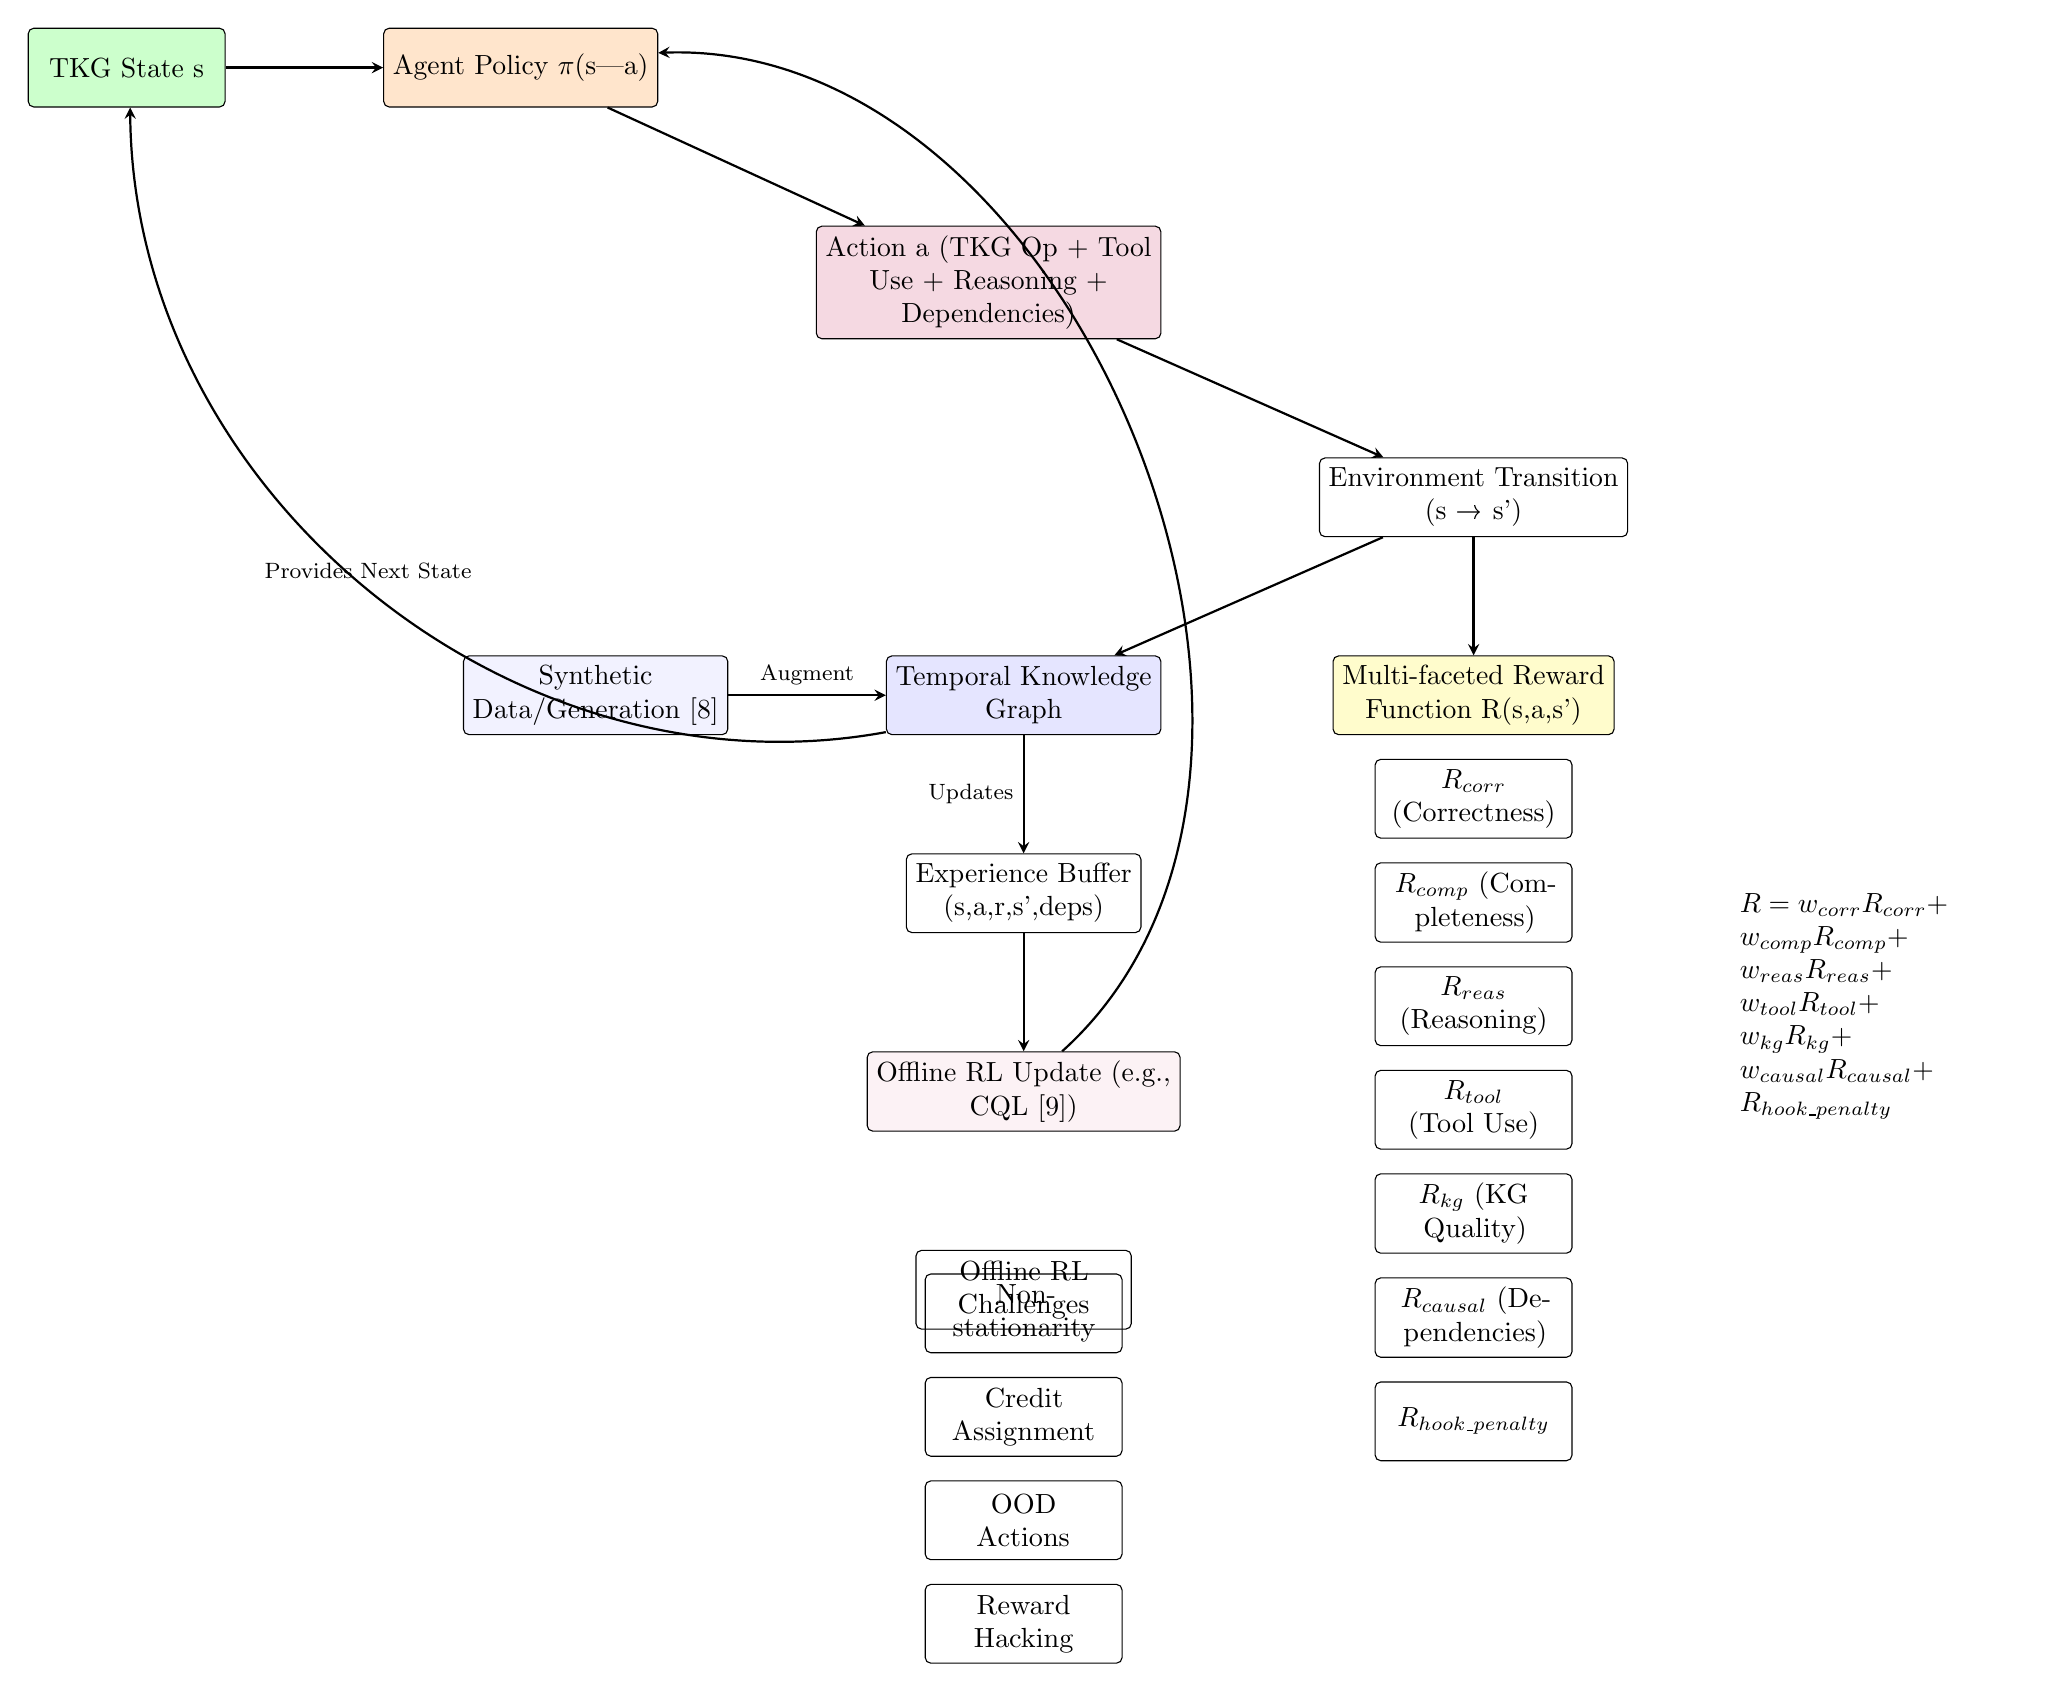
\begin{tikzpicture}[
    node distance=1.5cm and 2cm,
    box/.style={draw, minimum width=2.5cm, minimum height=1cm, align=center, rounded corners=2pt},
    state/.style={box, fill=green!20},
    agent/.style={box, fill=orange!20},
    action/.style={box, fill=purple!15},
    tkg/.style={box, fill=blue!10},
    reward/.style={box, fill=yellow!20},
    data/.style={box, fill=blue!5},
    rl/.style={box, fill=purple!5},
    arrow/.style={->, >=stealth, thick},
    note/.style={font=\footnotesize, align=center}
  ]
  
  % Main components
  \node[state] (tkg_state) {TKG State s};
  \node[agent, right=of tkg_state] (policy) {Agent Policy $\pi$(s|a)};
  \node[action, below right=of policy] (action) {Action a (TKG Op + Tool\\Use + Reasoning +\\Dependencies)};
  \node[box, below right=of action] (transition) {Environment Transition\\(s → s')};
  \node[tkg, below left=of transition] (tkg) {Temporal Knowledge\\Graph};
  \node[reward, below=of transition] (reward) {Multi-faceted Reward\\Function R(s,a,s')};
  
  % Reward components
  \node[box, below=0.3cm of reward, text width=2cm, align=center] (r_corr) {$R_{corr}$ (Correctness)};
  \node[box, below=0.3cm of r_corr, text width=2cm, align=center] (r_comp) {$R_{comp}$ (Completeness)};
  \node[box, below=0.3cm of r_comp, text width=2cm, align=center] (r_reas) {$R_{reas}$ (Reasoning)};
  \node[box, below=0.3cm of r_reas, text width=2cm, align=center] (r_tool) {$R_{tool}$ (Tool Use)};
  \node[box, below=0.3cm of r_tool, text width=2cm, align=center] (r_kg) {$R_{kg}$ (KG Quality)};
  \node[box, below=0.3cm of r_kg, text width=2cm, align=center] (r_causal) {$R_{causal}$ (Dependencies)};
  \node[box, below=0.3cm of r_causal, text width=2cm, align=center] (r_hook) {$R_{hook\_penalty}$};
  
  % Reward formula
  \node[box, right=of r_reas, text width=3.5cm, align=left, draw=none] (formula) {
    $R = w_{corr}R_{corr} +$\\
    $w_{comp}R_{comp} +$\\
    $w_{reas}R_{reas} +$\\
    $w_{tool}R_{tool} +$\\
    $w_{kg}R_{kg} +$\\
    $w_{causal}R_{causal} +$\\
    $R_{hook\_penalty}$
  };
  
  % Data and RL components
  \node[data, left=of tkg] (synth_data) {Synthetic\\Data/Generation [8]};
  \node[box, below=of tkg] (buffer) {Experience Buffer\\(s,a,r,s',deps)};
  \node[rl, below=of buffer] (offline_rl) {Offline RL Update (e.g.,\\CQL [9])};
  
  % Offline challenges
  \node[box, below=of offline_rl, text width=2.5cm, align=center, draw] (challenges) {Offline RL Challenges};
  \node[box, below=0.3cm of challenges.north, text width=2cm, align=center] (c1) {Non-stationarity};
  \node[box, below=0.3cm of c1, text width=2cm, align=center] (c2) {Credit Assignment};
  \node[box, below=0.3cm of c2, text width=2cm, align=center] (c3) {OOD Actions};
  \node[box, below=0.3cm of c3, text width=2cm, align=center] (c4) {Reward Hacking};
  
  % Connections
  \draw[arrow] (tkg_state) -- (policy);
  \draw[arrow] (policy) -- (action);
  \draw[arrow] (action) -- (transition);
  \draw[arrow] (transition) -- (tkg);
  \draw[arrow] (transition) -- (reward);
  \draw[arrow] (tkg) -- node[note, left] {Updates} (buffer);
  \draw[arrow] (buffer) -- (offline_rl);
  \draw[arrow] (offline_rl) to[bend right=70] node[note, left] {} (policy);
  \draw[arrow] (tkg) to[bend left=50] node[note, above] {Provides Next State} (tkg_state);
  \draw[arrow] (synth_data) -- node[note, above] {Augment} (tkg);
  
  \end{tikzpicture}
  \caption{Reinforcement Learning Flow in Arc: The system uses a multi-faceted reward function that incentivizes correctness, completeness, reasoning quality, effective tool use, knowledge graph quality, and proper causal dependency tracking. Agents learn from experience traces stored in the Temporal Knowledge Graph, with offline RL updates improving agent policies over time.}
  \label{fig:rl_flow}
\end{figure}

\begin{center}
\textit{Figure: Reinforcement Learning Flow in Arc - Training agents to collaborate effectively}
\end{center}

\begin{figure}[h]
  \centering
  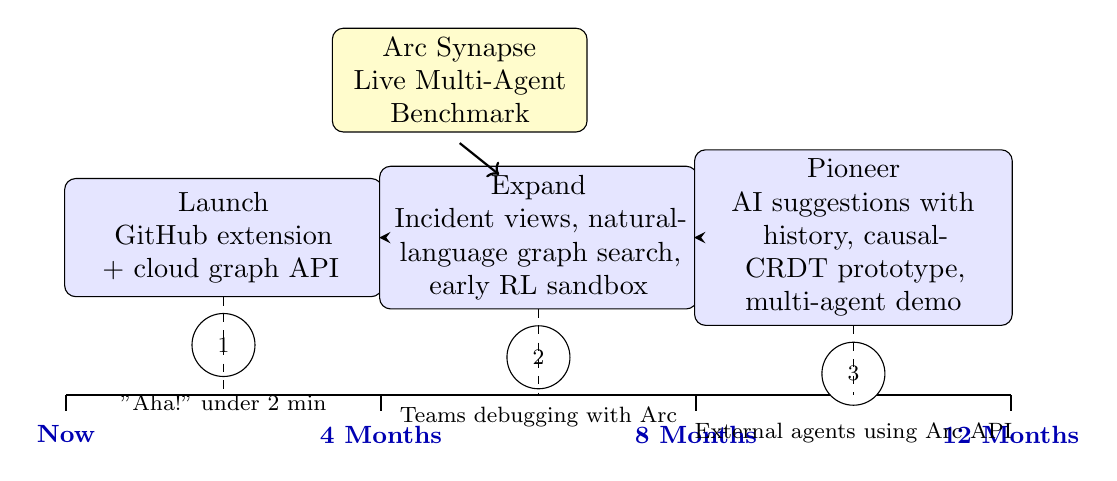
\begin{tikzpicture}[
    phase/.style={draw, rounded corners, fill=blue!10, minimum width=4cm, minimum height=1.5cm, text width=3.8cm, align=center},
    arrow/.style={->, >=stealth, thick},
    milestone/.style={draw, circle, fill=white, minimum size=0.8cm, inner sep=1pt, font=\footnotesize},
    timenode/.style={font=\small\bfseries, text=blue!70!black}
  ]
  
  % Timeline
  \draw[thick] (0,0) -- (12,0);
  
  % Phases
  \node[timenode] at (0,-0.5) {Now};
  \node[timenode] at (4,-0.5) {4 Months};
  \node[timenode] at (8,-0.5) {8 Months};
  \node[timenode] at (12,-0.5) {12 Months};
  
  % Launch Phase
  \node[phase] (launch) at (2,2) {Launch\\GitHub extension + cloud graph API};
  \node[milestone, below=0.2cm of launch] (m1) {1};
  \node[font=\footnotesize, below=0.1cm of m1] {"Aha!" under 2 min};
  
  % Expand Phase
  \node[phase] (expand) at (6,2) {Expand\\Incident views, natural-language graph search, early RL sandbox};
  \node[milestone, below=0.2cm of expand] (m2) {2};
  \node[font=\footnotesize, below=0.1cm of m2] {Teams debugging with Arc};
  
  % Pioneer Phase
  \node[phase] (pioneer) at (10,2) {Pioneer\\AI suggestions with history, causal-CRDT prototype, multi-agent demo};
  \node[milestone, below=0.2cm of pioneer] (m3) {3};
  \node[font=\footnotesize, below=0.1cm of m3] {External agents using Arc API};
  
  % Arrows
  \draw[arrow] (launch) -- (expand);
  \draw[arrow] (expand) -- (pioneer);
  
  % Timeline points
  \foreach \x in {0,4,8,12}
    \draw[thick] (\x,0) -- (\x,-0.2);
  
  % Connect phases to timeline
  \draw[dashed] (launch) -- (2,0);
  \draw[dashed] (expand) -- (6,0);
  \draw[dashed] (pioneer) -- (10,0);
  
  % Arc Synapse Event
  \node[draw, rounded corners, fill=yellow!20, text width=3cm, align=center] at (5,4) {Arc Synapse\\Live Multi-Agent\\Benchmark};
  \draw[->, thick] (5,3.2) -- (5.5,2.8);
  
  \end{tikzpicture}
  \caption{Arc Development Roadmap: A 12-month horizon showing key phases and milestones}
  \label{fig:roadmap}
\end{figure}

\begin{center}
\textit{Figure: Arc Development Roadmap - From initial launch to multi-agent coordination}
\end{center}

\section{Arc at a Glance}
Arc provides a shared, persistent, and semantically consistent foundation for collaborative AI software development. It integrates three core components, previously introduced, which work in concert to create an active world model of the software project:
\begin{itemize}
    \item \textbf{Temporal Knowledge Graph (TKG):} The system's collective memory, representing the evolving state of software artifacts, design decisions, and agent actions as a queryable, time-stamped graph.
    \item \textbf{Causal CRDT Layer:} Enables safe concurrent modifications by enforcing software-specific semantic dependencies derived from the TKG, preventing merges that would lead to invalid states.
    \item \textbf{Provenance-Driven RL:} Incentivizes agents not only for task completion but also for enriching and utilizing the TKG, fostering collaborative behavior and a deep understanding of context.
\end{itemize}
The illustrative example of upgrading OpenSSL across services highlights Arc's potential: Agent A refactors wrappers, Agent B updates API calls. Using Arc, Agent B can query the TKG for Agent A's progress. The Causal CRDT layer buffers Agent B's commit if dependencies (e.g., "Wrapper tests pass") aren't met. Both agents are rewarded for linking their work in the TKG, creating an understandable history.

\begin{figure}[h]
  \centering
  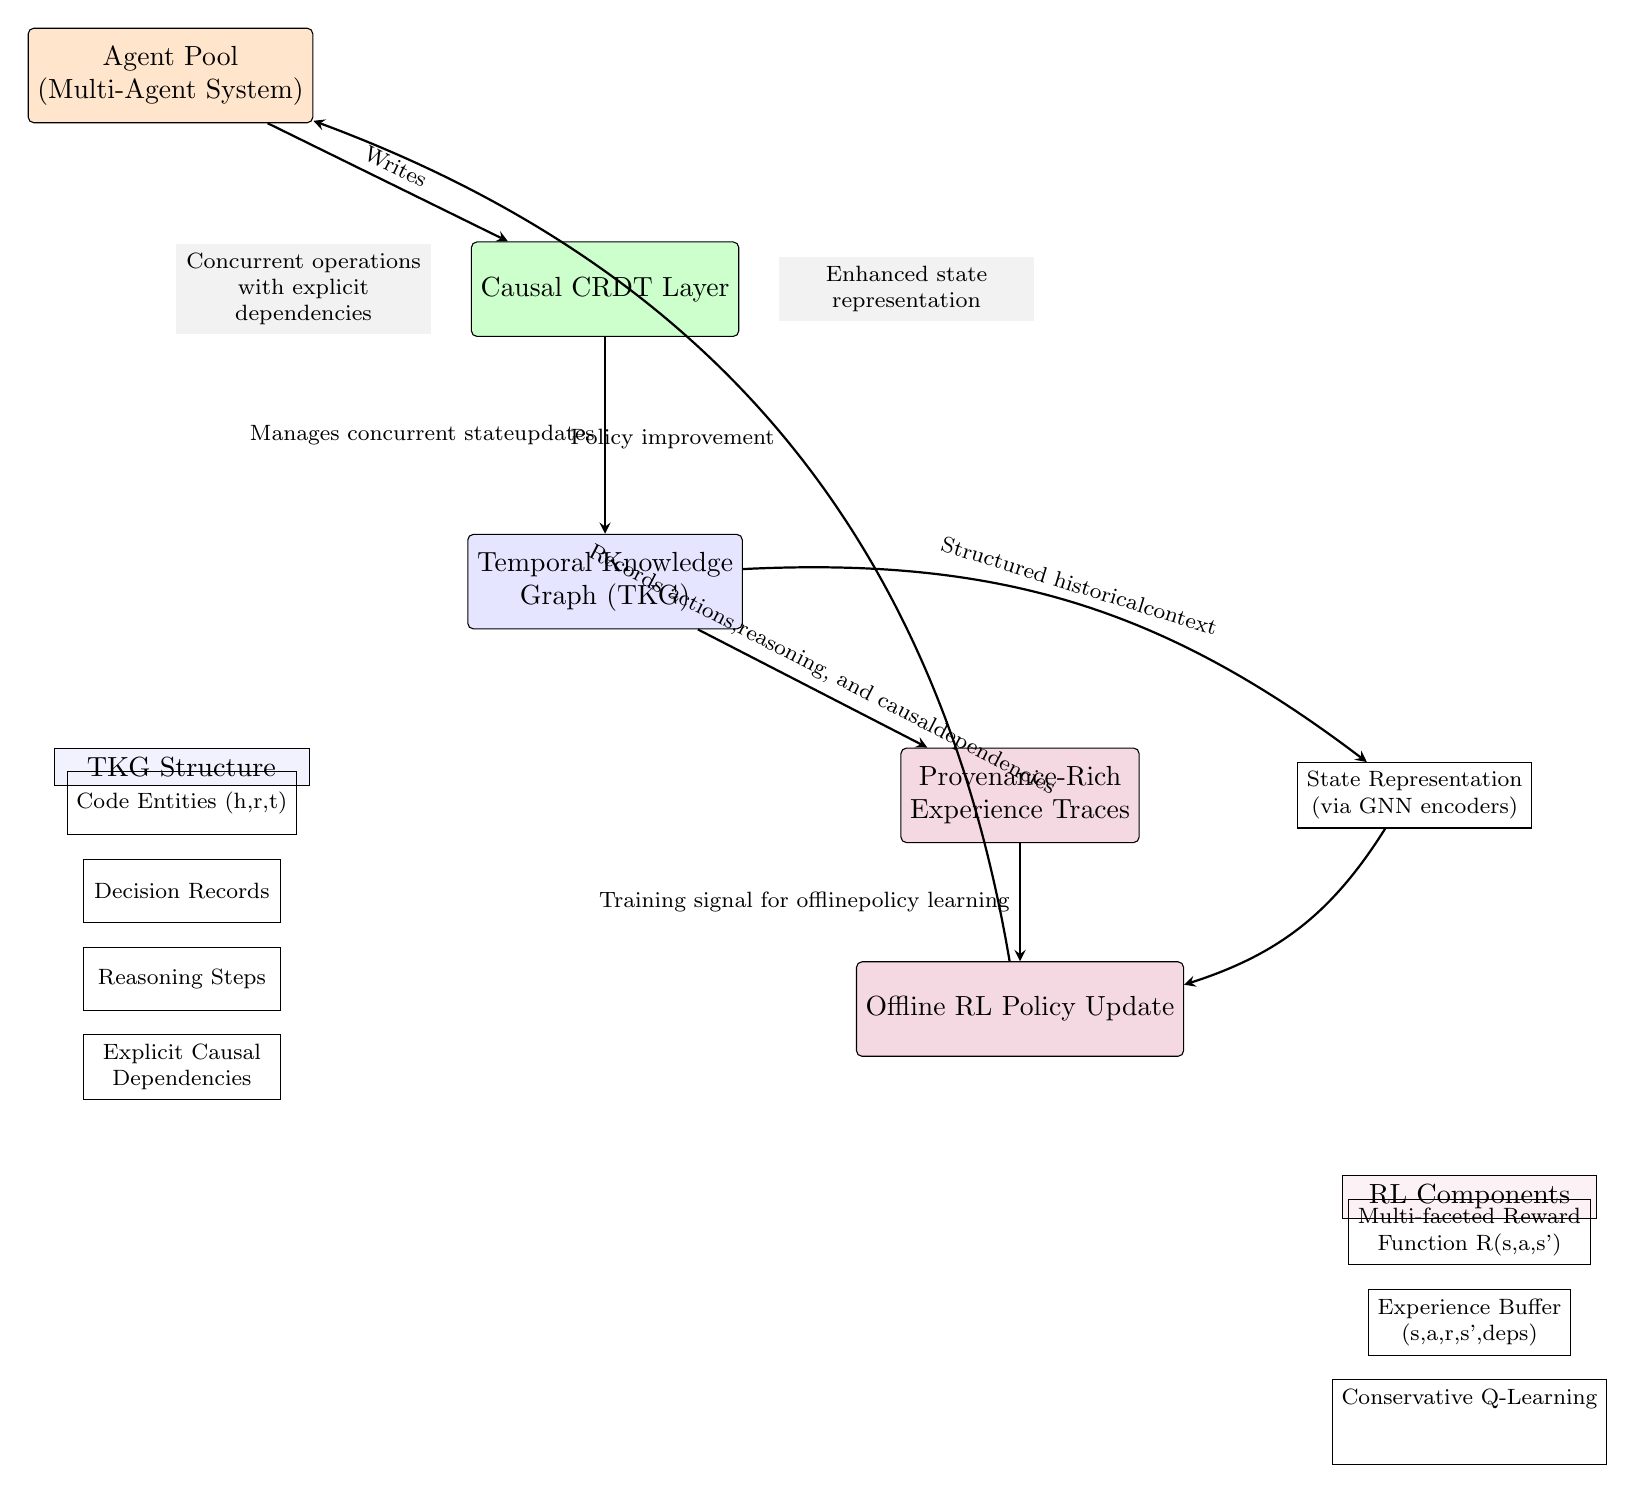
\begin{tikzpicture}[
    node distance=1.5cm and 2cm,
    box/.style={draw, minimum width=3cm, minimum height=1.2cm, align=center, rounded corners=2pt},
    agent/.style={box, fill=orange!20},
    tkg/.style={box, fill=blue!10},
    crdt/.style={box, fill=green!20},
    rl/.style={box, fill=purple!15},
    note/.style={draw=none, fill=gray!10, font=\footnotesize, align=center, text width=3cm},
    arrow/.style={->, >=stealth, thick},
    component/.style={draw, minimum width=2.5cm, minimum height=0.8cm, align=center, font=\footnotesize}
  ]
  
  % Main components
  \node[agent] (agent) {Agent Pool\\(Multi-Agent System)};
  \node[crdt, below right=of agent] (crdt) {Causal CRDT Layer};
  \node[tkg, below=2.5cm of crdt] (tkg) {Temporal Knowledge\\Graph (TKG)};
  \node[rl, below right=of tkg] (rl) {Provenance-Rich\\Experience Traces};
  \node[component, right=of rl] (state) {State Representation\\(via GNN encoders)};
  \node[rl, below=of rl] (offline) {Offline RL Policy Update};
  
  % TKG Components
  \node[draw, below left=of tkg, text width=3cm, align=center, fill=blue!5] (tkg_components) {TKG Structure};
  \node[component, below=0.3cm of tkg_components.north] (code) {Code Entities (h,r,t)};
  \node[component, below=0.3cm of code] (decisions) {Decision Records};
  \node[component, below=0.3cm of decisions] (reasoning) {Reasoning Steps};
  \node[component, below=0.3cm of reasoning] (dependencies) {Explicit Causal\\Dependencies};
  
  % RL Components
  \node[draw, below right=of offline, text width=3cm, align=center, fill=purple!5] (rl_components) {RL Components};
  \node[component, below=0.3cm of rl_components.north] (reward) {Multi-faceted Reward\\Function R(s,a,s')};
  \node[component, below=0.3cm of reward] (buffer) {Experience Buffer\\(s,a,r,s',deps)};
  \node[component, below=0.3cm of buffer] (q_learning) {Conservative Q-Learning\\[9]};
  
  % Connections
  \draw[arrow] (agent) -- node[above, sloped, font=\footnotesize] {Writes} (crdt);
  \draw[arrow] (crdt) -- node[left, font=\footnotesize] {Manages concurrent state\\updates} (tkg);
  \draw[arrow] (tkg) -- node[above, sloped, font=\footnotesize] {Records actions,\\reasoning, and causal\\dependencies} (rl);
  \draw[arrow] (rl) -- node[left, font=\footnotesize] {Training signal for offline\\policy learning} (offline);
  \draw[arrow] (offline) to[bend right=30] node[left, font=\footnotesize] {Policy improvement} (agent);
  \draw[arrow] (tkg) to[bend left=20] node[above, sloped, font=\footnotesize] {Structured historical\\context} (state);
  \draw[arrow] (state) to[bend left=20] node[right, font=\footnotesize] {} (offline);
  
  % Notes
  \node[note, right=0.5cm of crdt] {Enhanced state\\representation};
  \node[note, left=0.5cm of crdt] {Concurrent operations\\with explicit dependencies};
  
  \end{tikzpicture}
  \caption{Arc Architecture: The system integrates three key components: (1) A Temporal Knowledge Graph (TKG) that captures the evolving state of code artifacts, decisions, and agent actions; (2) A Causal CRDT layer that enables safe concurrent modifications by enforcing semantic dependencies; and (3) Provenance-driven Reinforcement Learning that rewards agents for generating and consuming causal context within the TKG.}
  \label{fig:arc_architecture}
\end{figure}

\begin{center}
\textit{Figure: Arc Architecture - Integrating Temporal Knowledge Graphs, Causal CRDTs, and Provenance-Driven RL}
\end{center}

\section{Problem Statement \& Research Gap}
The challenge is enabling multiple AI agents to collaboratively remember, reason about, and evolve software systems while maintaining architectural integrity and decision provenance.

\noindent\textbf{Research Question (RQ):} How can multiple RL coding agents maintain long-term architectural coherence while concurrently modifying a live codebase?

Existing approaches either (a) treat memory as passive RAG chunks, losing structural semantics, or (b) lock files to serialize edits, throttling parallelism. There is no system that offers structured, concurrent, provenance-aware memory tailored to code evolution. We formalize the gap as:
\begin{itemize}
  \item \textbf{P1 (Structure):} Absence of a canonical, query-efficient model linking commits, decisions, artifacts, and agent executions over time.
  \item \textbf{P2 (Concurrency):} Lack of write protocols (beyond basic CRDTs or locking) that respect higher-level semantic causal dependencies inherent in software evolution.
  \item \textbf{P3 (Learning):} Missing reward signals and learning frameworks that explicitly train agents to utilize shared historical context effectively and value the generation of explainable, historically consistent actions.
\end{itemize}

\section{Background and Related Work}
We synthesize advancements in distributed systems, knowledge representation, and reinforcement learning \cite{ref34}. We build on established concepts, proposing novel integrations for collaborative software evolution \cite{ref35}.

\subsection{Core Concepts}
\paragraph{Temporal Knowledge Graphs (TKGs)}
TKGs enhance knowledge graphs by adding temporal data, representing facts as quadruples $(h,r,t,\tau)$ with timestamps or intervals $\tau$ \cite{ref23}. Representation learning techniques model these temporal dynamics for forecasting and link prediction \cite{ref3,ref4,ref23,ref38}. TKGs offer a structured way to capture software evolution history over time \cite{ref37}.

\paragraph{Conflict-Free Replicated Data Types (CRDTs)}
CRDTs are data structures designed for distributed systems that guarantee eventual consistency without requiring complex consensus protocols, making them suitable for collaborative applications under network partitions \cite{ref5}. They achieve this through merge functions that are commutative, associative, and idempotent.

\paragraph{Reinforcement Learning (RL) for Code}
RL has been applied to various software engineering tasks, including code generation, optimization, and refactoring \cite{ref25,ref26}. Step-wise or offline RL approaches \cite{ref8,ref9,ref10} are particularly relevant for learning from interaction traces, potentially augmented with synthetic data \cite{ref8}, to train policies that map system states to actions.

\subsection{Related Work and Differentiation}
\begin{itemize}
  \item \textbf{Long Context LLMs \& Sequential Collaboration:} Frameworks like Chain-of-Agents \cite{ref11} and larger context windows help with long inputs but lack structured, concurrent workflows \cite{ref12,ref13}.
  \item \textbf{Causal Consistency Models:} Research on causal consistency in distributed systems \cite{ref14,ref15,ref24} informs our Causal CRDT design.
  \item \textbf{Graph-Based Agent Frameworks:} LangGraph \cite{ref18,ref19} and Graph-RAG \cite{ref20,ref21} use graphs for orchestration and retrieval; Arc uses the TKG as the shared, mutable world model and RL environment \cite{ref39}.
  \item \textbf{Graph-of-Thoughts(GoT}:GoT \cite{ref39} utilizes graph structures internally within a single LLM's reasoning process to explore different solution paths for complex problems. While powerful for individual agent reasoning, it doesn't address the shared, persistent, and concurrently modified memory challenges inherent in multi-agent software evolution that Arc targets.
  \item \textbf{Graph CRDTs:} Prior work on graph CRDTs and probabilistic causal contexts \cite{ref5,ref6,ref50} provides a foundation for our Causal CRDT.
  \item \textbf{RL on Dynamic/Temporal Graphs:} RL for temporal KGs \cite{ref46,ref47} and GNN representations \cite{ref15,ref31,ref36} guide our state‐encoding choices.
  \item \textbf{GitTemporalAI}: This concurrent work \cite{ref37} also leverages TKGs derived from Git history for repository intelligence, primarily focusing on analysis and querying by LLMs. Arc differentiates by using the TKG as a \textit{live, mutable environment} for \textit{concurrent agent action} mediated by Causal CRDTs and learned via RL, going beyond historical analysis to enable active, collaborative evolution.
  \item \textbf{Provenance Tracking:} Provenance mechanisms in storage systems \cite{ref16,ref17,ref27}, Software Heritage \cite{ref49}, and supply-chain frameworks like SLSA \cite{ref29,ref30} inspire our provenance integration.
  \item \textbf{Multi-Agent Collaboration \& Memory:} Dialogue-based frameworks (ChatDev \cite{ref43}, CAMEL \cite{ref44}), Generative Agents \cite{ref41}, and shared-memory MARL \cite{ref45, ref_srmt_arxiv} point to the need for a structured substrate.
\end{itemize}

\section{Proposed Approach: High-Level Architecture}
As illustrated in Figure \ref{fig:arc_architecture} above, Arc integrates three key components that work together to create a cohesive memory layer for software engineering.

\subsection{Temporal Knowledge Graph (TKG) as Environment}
The TKG serves as the shared world model and RL environment. \textit{Think of it as the project's collective, structured memory or logbook, capturing not just the code but the relationships between components, changes, and decisions over time.}
\begin{itemize}
  \item \textbf{Structure:} Software entities (services like \verb|auth-service|, \verb|payment-service|, files such as \verb|openssl_wrapper.c|, functions, commits, build dependencies, API contracts, agent assignments, and decisions) are nodes. Relationships (e.g., \verb|depends_on|, \verb|calls_api|, \verb|modified_by|, \verb|tested_by|) are typed edges with valid time intervals \cite{ref8}, representing the system's state. \cite{ref23}.
  \item \textbf{Query Capabilities:} Agents interact with the TKG via temporal graph queries \cite{ref_zep_lc}.
\begin{itemize}
    \item \textit{Example Query (Agent A):} "What services currently depend on \verb|libssl| and were last successfully built before my refactoring task started?" (Temporal snapshot query).
    \item \textit{Example Query (Agent B):} Show the history of changes to the \verb|PaymentAPI::process()| signature, and which agent initiated them." (Historical path query). Efficient indexing and partitioning techniques are crucial.
\end{itemize}
 \cite{ref24,ref32,ref33}.
  \item \textbf{RL State Representation:} Relevant TKG subgraphs, like Agent A's dependency graph, are encoded with GNNs for temporal graphs \cite{ref15,ref23,ref28,ref36}, producing vector states for policy networks.
\end{itemize}

\textbf{World-model view.} We treat the pair (TKG, $f_{\text{merge}}$) as a symbolic world model. The TKG provides the observable state $s$, while the Causal-CRDT merge function $f_{\text{merge}}(s, a)$ deterministically computes the next state if action $a$ is semantically valid. Because $f_{\text{merge}}$ is queryable before committing, an agent can ask counter-factual questions—e.g., "If I bump OpenSSL to 3.0, which services will violate dependency tests?". While the goal is to receive answers rapidly (e.g., within milliseconds for common queries), achieving this for massive, evolving TKGs relies on ongoing research into highly scalable graph database technologies, efficient indexing, partitioning techniques \cite{ref24, ref32, ref33}, and query optimization. This elevates Arc beyond large-context retrieval toward model-based planning in software-engineering domains.

\subsection{Causal CRDT Layer}

We propose an operation-based Causal CRDT to manage concurrent writes while preserving semantic dependencies. Standard CRDTs ensure concurrent text edits eventually merge, but they don't understand if merging breaks the build or violates an API contract. Our Causal CRDT layer adds software-specific "guardrails," derived from the TKG, to prevent merges that, while textually valid, would be semantically incorrect in the context of the software project.

\begin{itemize}
  \item \textbf{Design:} Each operation has dependency metadata (`deps`) and a vector clock. Merges happen when all dependencies and causal predecessors are satisfied \cite{ref5,ref14,ref15,ref24}, otherwise they are buffered.
      \begin{itemize}
          \item \textit{Example Operation (Agent B):} \verb|Op:UpdateAPISignature(PaymentAPI)| (ensuring Agent A's foundational refactor is committed before the API depending on it is changed). Merges (applying operations to the shared state) occur only when all vector clock predecessors \textit{and} explicit TKG-derived dependencies are satisfied \cite{ref9, ref20, ref21, ref22}. Operations with unmet dependencies are buffered (See Figure \ref{fig:causal_dependency} above).
      \end{itemize}

  \item \textbf{Differentiation:} Its novelty is in enforcing deterministic, application-specific causal invariants critical for software evolution (e.g., "a service cannot deploy if dependent libraries fail tests," "an API change requires updating all callers"). Unlike structural CRDTs or probabilistic approaches, Arc leverages the live TKG state during the merge protocol to define and check semantic invariants via metadata, ensuring correctness beyond eventual consistency.
While fine-grained Abstract Syntax Tree (AST) level CRDTs pose additional challenges, our initial focus is on file-level operations guided by TKG semantics. Furthermore, complex semantic checks like full test suite execution are infeasible during the synchronous merge. Our protocol thus prioritizes \textit{efficiently checkable invariants}. For example, an invariant like "API signature (name, arity, parameter types) must match the TKG-defined contract for \verb|PaymentAPI::process()|" can be checked synchronously by querying the TKG. In contrast, a full behavioral test asserting "all existing callers of \verb|PaymentAPI::process()| still function correctly post-change" would typically be deferred to asynchronous CI gates, which are themselves informed by TKG provenance. This approach allows concurrent edits while respecting the rules of software development.
\end{itemize}

\subsection{Step-Wise Reinforcement Learning (RL) Loop}
Agents learn optimal policies for evolving codebases within the TKG environment using offline RL from interaction traces \cite{ref12, ref19}. \textit{The goal isn't just to teach agents to write code, but to teach them how to be effective members of a collaborative team, using the shared memory to coordinate and understand context.} Each trace step contains the state, action, reward, next state, and causal dependencies: (s,a,r,s$'$,deps). As illustrated in Figure \ref{fig:rl_flow} above, this process creates a learning flywheel.

\begin{itemize}
     \item \textbf{Multi-Component Reward:} The reward function $R$ guides agents to become effective collaborators by considering multiple factors beyond task completion.
$R = R_{\text{corr}} + R_{\text{comp}} + R_{\text{reas}} + R_{\text{tool}} + R_{\text{kg}} + R_{\text{causal}}$

It consists of several components:
    \begin{itemize}
        \item  (Correctness): Reward for code changes passing tests, static analysis, and type checks, with penalties for build failures or regressions. Penalties for build failures or introducing regressions.
        \item  (Completion): Reward for making progress towards the overall goal (e.g., percentage of services successfully migrated from the old OpenSSL version).
        \item  (Reasoning Quality): Reward for generating clear, logical intermediate reasoning steps or plans (potentially evaluated by another LLM or based on plan structure).
        \item  (Tool Use Efficiency): Reward for selecting appropriate tools (compiler, test runner, refactoring engine) and using them effectively.
         \item  (TKG Enrichment): \textbf{Crucially, reward for enriching the TKG with valuable provenance.} \textit{This incentivizes agents to "document their work" by linking their actions to reasons within the shared memory, making the system's history understandable.}\textit{Example:} Agent B gets a reward for adding an edge \verb|updates_dependency_introduced_by| linking its API change node to Agent A's earlier commit node in the TKG. This explicitly captures the rationale.
         \textit{Note: Simply counting new edges ($R_{kg}$) could potentially be gamed by agents adding trivial links. Future refinements will explore quality-based provenance rewards, perhaps using link prediction models trained on human-validated traces or rewarding edges that resolve specific TKG consistency queries.}
        \item  (Causal Coordination): Reward reflecting an action's interaction with the Causal CRDT layer's dependency constraints. Positive reward is granted when an action satisfies dependencies that unblock \textit{other agents'} buffered operations (promoting flow); negative reward (or cost) is incurred for actions that become buffered themselves due to unmet prerequisites or contribute to potential causal cycles (discouraging deadlock).
        \begin{itemize}
            \item \textit{Example:} Agent A receives a positive causal boost upon committing its refactor, as this unblocks Agent B's dependent API update operation.
        \end{itemize}
    \end{itemize}
    \item \textbf{Learning Algorithm:} Our primary learning strategy leverages offline RL algorithms (e.g., CQL \cite{ref46}, IQL \cite{ref11}, OREO \cite{ref48}) for their sample efficiency, training policies ($\pi(a\mid s)$) on accumulated interaction traces. On-policy fine-tuning (e.g., using PPO) based on live interactions within the Synapse environment is a potential subsequent step for further optimization, considered future work for the initial validation phase. Initial traces for bootstrapping the learning process may be sourced from existing human commit histories, curated datasets of code evolution, or through a human-in-the-loop phase where expert developers guide initial agent actions.
    \item \textbf{Flywheel Effect:} Enhanced policies enable agents to produce more effective actions and richer provenance traces. These traces yield higher-quality data for subsequent offline RL training, fostering a self-improving cycle where agents excel at collaborative, long-term software evolution.
\end{itemize}

\section{Practical Considerations \& Industry Impact}
While Arc presents a powerful vision, practical adoption requires addressing several considerations:

\begin{itemize}
    \item \textbf{Integration:} Integration with existing developer ecosystems is key. This requires developing adapters for common Git workflows (e.g., interpreting Arc operations as Git commits with rich metadata), hooks for CI/CD pipelines (e.g., validating TKG consistency before deployment), and potentially IDE plugins for visualizing TKG context and agent activity.
    \item \textbf{Scalability:} Real-world repositories can be massive. Efficient TKG storage (e.g., using specialized graph databases \cite{ref43, ref44}), indexing, and query optimization are paramount. Vector clock and dependency metadata compaction strategies are needed.
    \item \textbf{Human Oversight:} Mechanisms for human developers to inspect the TKG, understand agent decisions via provenance trails, override actions, and guide the RL process are essential for trust and safety \cite{ref15, ref16, ref42}. Visualization tools are key.
\end{itemize}
Addressing these points enables substantial industry impact:
\begin{itemize}
    \item \textbf{Accelerated Large-Scale Changes:} Tasks like the OpenSSL upgrade example, major refactorings, or framework migrations, which are currently slow and error-prone, could be significantly accelerated by coordinated AI agents.
    \item \textbf{Reduced Integration Conflicts:} \\Causal CRDTs and shared TKG awareness minimize broken builds and integration issues common in parallel development.
    \item \textbf{Enhanced Maintainability:} The provenance-rich TKG acts as living documentation, making it easier for both humans and AI agents to understand legacy code and the rationale behind past changes.
    \item \textbf{Autonomous Systems:} Arc provides a foundation for more autonomous AI agents capable of long-term maintenance, proactive bug fixing, and continuous modernization of software systems.
\end{itemize}


\section{Research Agenda \& Open Challenges}
Arc opens research frontiers at the intersection of distributed systems, program provenance, and reinforcement learning. Its success hinges on collaborative innovation to address the following open challenges, presented here as explicit invitations for collaboration:

\begin{itemize}
  \item \textbf{Formal Foundations:} Key questions include establishing safety and liveness guarantees for Causal CRDTs under real-world branching patterns and defining how semantic invariants (e.g., build determinism, API compatibility) can be expressed in merge-able logic. \emph{Hypothesis:} Causal CRDTs will reduce semantic merge conflicts by $\ge$30\,\% on the Synapse benchmark versus standard CRDTs. \emph{Call for collaboration:} Formal-methods researchers for distributed protocol proofs.

  \item \textbf{Scalability \& Performance:} Critical challenges involve mitigating TKG query latency in interactive RL loops (via caching, state abstraction, or predictive prefetching), adapting TKG schemas to evolving artifact types while maintaining query consistency, sustaining sub-second queries on graphs exceeding $10^{8}$ edges, and compressing vector-clock metadata without violating causality. \emph{Call for collaboration:} Systems engineers experienced with high-throughput graph databases or CRDT optimization, particularly for temporal graph storage and delta-propagation techniques.

  \item \textbf{Advanced Reinforcement Learning:} We aim to design tractable graph-centric state representations for offline RL and explore hierarchical RL to bridge fine-grained edits with macro-architectural tasks. \emph{Research focus:} Curriculum learning on progressively larger TKG subgraphs and reward decomposition ($\{R_{\text{corr}},R_{\text{comp}},R_{\text{prov}},R_{\text{causal}}\}$) tuned via population-based training. \emph{Call for collaboration:} RL scholars interested in latent-graph policies and combinatorial action spaces for provenance-driven agents.

  \item \textbf{Human–Agent Interaction:} Core questions are how to best design visual abstractions for million-edge causal chains within the TKG and develop just-in-time human oversight mechanisms for resolving highly ambiguous merges. \emph{Opportunity:} Adapt existing provenance-graph UIs \cite{ref15, ref16} for deployment as VS Code extensions. \emph{Call for collaboration:} HCI and visualization researchers, and maintainers of developer-tooling plugins.

  \item \textbf{Generalisation \& Transfer:} We seek to determine if agent embeddings of causal code traces can transfer across programming languages and whether meta-learning can accelerate adaptation for tasks like migrating a security patch from Java to Python. \emph{Call for collaboration:} Experts in few-shot learning and multilingual code-analysis.

  \item \textbf{Cross-Modal Integration:} Key challenges include reconciling heterogeneous signals—such as issue trackers, design documents (ADRs), and log traces—into a unified TKG schema, and developing retrieval strategies that surface the optimal context slice to an agent within latency constraints. \emph{Call for collaboration:} Information-integration researchers and practitioners of large-scale RAG systems.

  \item \textbf{Limitations \& Failure Modes:} Known risks include TKG query latency bottlenecking agent planning, offline RL sensitivity to historical data bias, and potential Causal CRDT deadlocks under complex circular semantic dependencies. \emph{Mitigation focus:} Investigating timeouts, dependency height limits, and designated deadlock "breakers" (human or AI) informed by TKG cycle detection, alongside runtime monitoring and adversarial stress testing. \emph{Call for collaboration:} Reliability engineers and researchers in formal verification of RL agents.
\end{itemize}

The development of Arc is envisioned as an open, collaborative effort. We actively seek partners from academia and industry with expertise in the aforementioned areas. By engaging with the SYNAPSE benchmark (Section \ref{sec:synapse}) and contributing to these core ideas, we can collectively transform software evolution from a fragile, sequential process into a consistent, multi-agent endeavor. We believe building this foundational memory layer is critical for the future of AI in software engineering.

\section{Synapse Benchmark}
\label{sec:synapse}

\subsection{V1 Task Definition}
\textbf{Scenario.}
Two RL-driven coding agents, each powered by Arc, must upgrade \texttt{OpenSSL} from v1.1 to v3.0 across a \emph{synthetic microservice monorepo} containing 20 heterogeneously-typed services (14 Python + 6 Java).  The synthetic repository comprises approximately 8-12 KLOC across services. The full test suite (\texttt{pytest} + \texttt{mvn verify}) typically completes in under 15 minutes on standard CI hardware (e.g., 4-core GitHub Actions runner).
The repository is generated from a parameterised template inspired by industry testbeds such as \textsc{Sock Shop} and \textsc{Hipster Shop}; each service exposes either gRPC or REST endpoints and has transitive dependencies on \texttt{libssl}.  Dependency graphs and CI pipelines are committed into the Temporal Knowledge Graph (TKG) at \texttt{t\_0}.

\smallskip
\noindent\textbf{Goal.}
Within an 8-hour wall-clock budget and a 1\,000-action cap per agent, perform the upgrade while preserving all unit $\&$ integration tests (\texttt{pytest -c -q} for Python, \texttt{mvn verify} for Java) and maintaining a clean CI run.

\subsection{Environment \& Infrastructure}
\begin{itemize}
    \item \textbf{Execution Harness.} Docker Compose + Bazel build farm (local or K8s) orchestrates parallel builds and test runs; a Git server with pre-receive hooks provides ground-truth CI verdicts.
    \item \textbf{Arc Instance.} A single logical replica hosts the TKG and Causal CRDT engine.  Agents interact solely via Arc’s gRPC API—no hidden channel exists.
    \item \textbf{Observation/Action Space.}
          Agents receive \texttt{(diff, TKG\_snapshot, build\_status)} tuples and may issue atomic CRDT operations: \texttt{edit(file)}, \texttt{commit(msg)}, \texttt{merge(branch)}, \texttt{query(TKG)}, etc.
    \item \textbf{RL Algorithm.} Agents are trained primarily using offline RL (e.g., CQL/IQL) on previously collected interaction data within the Synapse environment. A curriculum schedule is employed: warm-start training on single-service upgrades, then advance to the full 20-service monorepo dataset once $\ge$80\,\% success is achieved on simpler tasks. (On-policy fine-tuning with algorithms like PPO is reserved for future investigation, potentially in V3).
\end{itemize}

\subsection{Metrics}
\begin{enumerate}
    \item \textbf{Task Completion Rate \& Latency}—fraction of services upgraded + median completion time.
    \item \textbf{Integration Errors}—CI failures attributable to semantic regressions (build or runtime).
    \item \textbf{Concurrent Throughput}—95th-percentile number of non-conflicting CRDT commits per minute.
    \item \textbf{Provenance Quality}—TKG density of causal edges (\verb|depends_on|, \verb|triggered_by|, \verb|resolved_by|) \emph{validated} against ground-truth commit history; manual spot-checks for interpretability.
    \item \textbf{Causal Conflict Resolution}—ratio of semantic conflicts auto-resolved by the Causal CRDT vs.\ rolled back or surfaced to humans.
\end{enumerate}

\subsection{Baselines}
\begin{description}
    \item[Single-Agent (Long Context)] State-of-the-art model long context model with a 200k+ token window (Claude 3.7 Sonnet, Gemini 2.5 Pro, GPT 4.1); mirrors SWE-bench evaluation style.
    \item[Multi-Agent (File Locking)] Two agents use coarse file-level locks; high contention expected.
    \item[Multi-Agent (Standard CRDT)] Automerge-style CRDT without semantic guards; syntactic merge success yet high logical error rate.
    \item[Multi-Agent (RAG + Scratchpad)] Each agent queries a vector store of code chunks plus a private scratchpad, similar to Graph-of-Thoughts orchestration.
    \item[Ablations] (i) Arc with Causal CRDT disabled (falls back to locking); (ii) Arc with TKG replaced by naive RAG.
\end{description}

\subsection{Reward Function}
The reward function for the SYNAPSE benchmark combines dense and sparse signals, directly reflecting the multi-component reward $R$ detailed in Section 5.3. It is formulated as:
$R = w_{\text{corr}}R_{\text{corr}} + w_{\text{comp}}R_{\text{comp}} + w_{\text{reas}}R_{\text{reas}} + w_{\text{tool}}R_{\text{tool}} + w_{\text{kg}}R_{\text{kg}} + w_{\text{causal}}R_{\text{causal}}$
where:
\begin{itemize}
    \item $R_{\text{corr}}$ (Correctness): Based on tests passing, static analysis, type checks.
    \item $R_{\text{comp}}$ (Completion): Progress towards the OpenSSL upgrade goal.
    \item $R_{\text{reas}}$ (Reasoning Quality): Quality of intermediate reasoning (if applicable).
    \item $R_{\text{tool}}$ (Tool Use Efficiency): Efficient use of build/test tools.
    \item $R_{\text{kg}}$ (TKG Enrichment): Number and quality of new causal edges added to TKG.
    \item $R_{\text{causal}}$ (Causal Coordination): Positive for unblocking operations, negative for causing buffered operations or deadlocks.
\end{itemize}
The weights ($w_i$) will be optimized through techniques like population-based training to balance task velocity with the richness of provenance and collaborative behavior. Initial settings will prioritize correctness and completion, with increasing emphasis on TKG enrichment and causal coordination as agent capabilities mature.

\subsection{Success Criteria}
Arc aims to achieve \textbf{(i)} $\ge$95\,\% service upgrade rate, \textbf{(ii)} $>$50\,\% fewer integration errors, and \textbf{(iii)} $\ge$2$\times$ higher concurrent throughput than locking \emph{and} standard-CRDT baselines, while producing a TKG whose causal-edge density is within 10\,\% of ground-truth links.

\subsection{Proposed Roadmap}

\textbf{V2} will replace the synthetic mono repo with  \textsc{SWE-bench} subset issues that require multi-file patches, extending from single-agent to cooperative multi-agent repairs. \textbf{V3} plans to introduce cross-language refactors (Python $\leftrightarrow$ Go) and partial offline-RL fine-tuning, aligning with emerging multi-agent toolchains.

\section{Conclusion}
AI-generated code presents both opportunity and risk: accelerated development alongside "context collapse" where rationale becomes opaque. Current LLM agents hit a "transient-context ceiling," struggling with causal understanding across multiple commits. They may generate code efficiently but fail to preserve architectural intent and the crucial "why" behind changes. Arc addresses this by integrating Temporal Knowledge Graphs, Causal CRDTs, and Provenance-Driven RL into a cohesive memory plane.

We anticipate significant impact: accelerating large-scale refactorings, enabling self-healing systems, and reducing integration conflicts. The SYNAPSE benchmark provides a concrete validation path, but realizing this vision requires collaborative effort. We invite the research community to engage with these ideas and help build the future of structured, concurrent, and provenance-aware collective AI memory for software engineering—moving beyond transient context toward a new generation of AI-assisted development.

\section*{Acknowledgments}
We thank the research community for valuable discussions that have shaped this position paper. We welcome collaboration on the open challenges outlined in our research agenda. For inquiries about Arc or potential collaborations, please contact \texttt{Jarrod@arc.computer}.

\bibliographystyle{abbrvnat}
\bibliography{references}

\clearpage
\section*{Glossary}

\begin{description}
\item[Temporal Knowledge Graph (TKG)] A dynamic graph structure that captures the evolution of code, design decisions, requirements, agent actions, and their causal interdependencies over time. Unlike static code graphs, TKGs represent facts as quadruples $(h,r,t,\tau)$ with timestamps or intervals $\tau$.

\item[Causal CRDT] An extension of Conflict-free Replicated Data Types (CRDTs) that enforces semantic invariants derived from the TKG during concurrent operations. These invariants preserve crucial dependencies like build order and API contracts, preventing logical conflicts while allowing parallel edits.

\item[Provenance-Driven Reinforcement Learning] A learning approach where agents are rewarded for generating and consuming causal context within the TKG—linking changes to requirements, documenting decisions, and unblocking other agents—fostering truly collaborative and auditable AI systems.

\item[SYNAPSE Benchmark] A real-world benchmark for evaluating multi-agent engineering systems, where two AI agents must upgrade OpenSSL across a microservice monorepo while maintaining build integrity and test coverage.

\item[Vector Clock] A data structure used in distributed systems to establish a partial ordering of events. In Arc, vector clocks help track causal relationships between operations performed by different agents.

\item[Architectural Decision Records (ADRs)] Structured documents that capture important architectural decisions made during the development process, including context, consequences, and alternatives considered.

\item[Context Collapse] The phenomenon where critical "why" context is scattered across different tools and systems, making it difficult to understand the rationale behind code changes, especially as AI accelerates code generation.

\item[Provenance Gap] The challenge of tracking the origin, requirements, and verification status of AI-generated code, which becomes increasingly important as AI generates more code with less human oversight.

\item[Coordination Chaos] The problem that arises when multiple AI agents (and humans) work on the same codebase without a common world model, introducing conflicts and inconsistencies.

\item[World Model] A comprehensive representation of a system that captures not just its current state but also the causal relationships and dynamics that govern how it evolves over time.
\end{description}


\vspace{0.5cm}
\begin{center}
\rule{0.5\textwidth}{0.5pt}
\vspace{0.5cm}

\qrcode[height=1.5in]{https://arc.computer}
\\ \vspace{0.3cm}
\textit{Learn more about Arc at \href{https://arc.computer}{arc.computer}}
\end{center}
\end{document}